\glspl{MSR} possess unique characteristics which render existing \gls{LWR}
analysis software inappropriate for \gls{MSR} analysis. Legacy \gls{LWR}
software typically scale poorly on modern high-performance computing
clusters and do not support complex geometries beyond regular \gls{LWR} fuel
assembly lattices. Furthermore, \glspl{MSR} feature strong multiphysics
coupling which force segregated solvers into taking smaller timesteps to
maintain accuracy. This chapter provides a brief history of \glspl{MSR},
followed by a discussion of the challenges in \gls{MSR} multiphysics modeling
for reactor accident analysis. Next, this chapter presents a literature review
of existing multiphysics simulation software developed for \glspl{MSR}
analysis. This work focuses software for analysing short-term reactor dynamics
which requires the ability to accurately simulate various transient scenarios
such as reactor start-up and coast-down, load-following operations,
steady-state operation, and accident analysis. Long-term dynamics such as fuel
burnup and structural corrosion fall outside the scope of this work. Lastly,
this chapter reviews the existing capabilities of Moltres, the MSR simulation
software to be developed in this work.

\section{Molten Salt Reactors}

The first \gls{MSR}, named the \gls{ARE}, dates back to the 1940s
as part of the US Aircraft Nuclear Propulsion program
\cite{rosenthal_molten-salt_1970}. Researchers recommended molten fluoride
salts in particular for high uranium solubility, chemical stability, low vapor
pressure even at high temperatures, good heat transfer properties,
resistance against radiation damage, and reduced corrosive effects on some
common structural material \cite{rosenthal_molten-salt_1970}. They
subsequently built the 2.5 MW$_{\text{th}}$ ARE reactor at \gls{ORNL}, where
it achieved criticality on November 1954 and generated 100 MWh over nine days.
The reactor ran on enriched uranium in a molten salt mixture of NaF,
ZrF$_4$, and UF$_4$ with BeO neutron moderators. The aircraft program
ultimately never came to fruition as the development of intercontinental
ballistic missiles effectively eliminated the need for long-range
nuclear-powered bomber aircraft.

However, the successful demonstration of the \gls{ARE} spurred further
research into adapting \glspl{MSR} for civilian power generation
\cite{rosenthal_molten-salt_1970}. One key finding from the
research was that the thorium fuel cycle had a better breeding ratio than the
$^{238}$U-to-$^{239}$Pu fuel cycle in thermal-spectrum reactors.
Ultimately, these efforts culminated in the design, construction, and
successful operation of the \gls{MSRE}, a graphite-moderated thermal
\gls{MSR}. The \gls{MSRE} had a
graphite-moderated design with a LiF-BeF$_2$-ZrF$_4$-UF$_4$ fuel salt mixture,
initially rated at 10 MW$_{\text{th}}$ but later restricted to 8
MW$_{\text{th}}$ due to a miscalculation of heat transfer capabilities
\cite{haubenreich_experience_1970}. In January 1969, the \gls{MSRE} became the
first reactor to run on $^{233}$U fuel.

Building on their experience with the \gls{MSRE}, \gls{ORNL} proposed a
new program for the construction and operation of a demonstration reactor
based on the \gls{MSBR} concept that they had
developed \cite{macpherson_molten_1985}. The \gls{MSBR} is a thermal-spectrum,
single fluid reactor with fertile $^{232}$Th isotopes mixed directly into the
FLiBe molten salt for $^{233}$U breeding \cite{gehin_liquid_2016}. Like the
\gls{MSRE}, the \gls{MSBR} relies on continuous online reprocessing to add
fertile material and remove fission product neutron poisons. Researchers
estimated the doubling time (the minimum amount of time required to produce
enough fissile material to start up another \gls{MSBR}) to be
approximately 22 years. However, \gls{ORNL} failed to secure funding for the
new program in their two attempts in 1972 and 1974. Nevertheless, from a
technical perspective, two independent
technology evaluation and design studies of the \gls{MSR} had reported
favorably on the promise of the system \cite{macpherson_molten_1985}.

In spite of this setback, research into \glspl{MSR} continued through the late
1970s. In 1980, \gls{ORNL} published a report describing a new \gls{MSR}
concept, called the \gls{DMSR} \cite{gehin_liquid_2016} with denatured
$^{235}$U fuel (i.e. low-enriched uranium). The \gls{ORNL} researchers
developed this design in response to the fuel reprocessing restrictions
introduced by President Ford in 1976. The \gls{DMSR} would operate as a
once-through
converter system without fuel reprocessing. While the fuel consists of 19.75
\% high-assay low-enriched uranium, the initial core loading includes thorium
to boost its conversion ratio throughout its lifetime. It has a continuous
online feed consisting of \gls{HALEU} to maintain criticality, and denatured
$^{235}$U to keep uranium enrichment levels below nuclear non-proliferation
policy thresholds. The design also includes a gas sparging system for removing
gaseous fission products, while noble metals plate out onto the walls of
the coolant loop. The older \gls{MSBR} design had a significant drawback; the
extensive neutron damage in the graphite moderator necessitated frequent
replacement (every four years) throughout its operational lifetime. The
\gls{DMSR} avoids this issue by running on a lower power density while
maintaining
the overall power output of 2250 MW$_{\text{th}}$. As a result, researchers
projected that the graphite moderator would last for the entirety of the
\gls{DMSR}'s design lifetime.

A concurrent program at the UK Atomic Energy Authority led the
development of a 2500 MW$_{\text{e}}$ lead-cooled Molten Chloride Fast Reactor
concept \cite{smith_assessment_1974}. It is a dual fluid system,
with separate loops for the fuel salt and the blanket salt. The blanket is a
1 m-wide tank surrounding the core. The absence of moderators and the choice
of chloride over fluoride salt resulted in a relatively hard neutron spectrum
which favors $^{239}$Pu breeding over the thorium cycle. The UK researchers
performed some experiments to study molten salt chemistry but they did not
build reactor prototypes. The UK program eventually shut down just like its
US counterpart partly due to the successful demonstration of the Prototype
Fast Reactor which had achieved criticality in 1974.

Following a lull lasting through the late 20th century, researchers at
\gls{CNRS} began research into \glspl{MSR} in 1997
\cite{heuer_simulation_2010}. Starting from the \gls{MSBR} design, they
performed parametric studies based on safety, breeding, and
other performance metrics \cite{mathieu_thorium_2006}. Their efforts
culminated in the \gls{MSFR} concept, a fast-spectrum breeder \gls{MSR}
designed to run on the thorium fuel cycle \cite{merle_optimized_2007}. In
2008, the Generation IV International Forum highlighted the \gls{MSFR} among
other \gls{MSR} designs for further development \cite{gif_generation_2008}.
The \gls{MSFR} has also benefited from collaborative research through three
European-funded projects, the \gls{EVOL} \cite{euratom_final_2015},
\gls{SAMOFAR} \cite{kloosterman_20_2017}, and \gls{SAMOSAFER}
\cite{cordis_severe_nodate} projects. Under the \gls{EVOL}
project, researchers further optimized the \gls{MSFR} design based on
neutronic and thermal-hydraulic safety analyses. They also diversified
start-up fuel options beyond the original $^{233}$U-based fuel composition to
include $^{235}$U, $^{239}$Pu, and \gls{TRU}, and established fuel
reprocessing schemes for the \gls{MSFR}. The \gls{SAMOFAR} project, which
started approximately two years after the end of the \gls{EVOL} project,
supported more comprehensive safety assessments of the reactor and the
reprocessing plant, and funded a number of experiments for validation of the
\gls{MSFR}'s safety features. The ongoing \gls{SAMOSAFER} project funds further
research activities with the goal of achieving modeling, analysis, and
design improvements on various aspects of \gls{MSR} operation and safety. As
opposed to the channel-type design of the \gls{MSRE} and \gls{MSBR}, the
\gls{MSFR} reactor core consists of a single, large channel through which the
salt flows as shown in Figure \ref{fig:msfr}. The omission of graphite channels
avoids operational and design issues associated with graphite neutron damage
and parasitic absorption and results in
a harder neutron spectrum than the \gls{MSRE} and \gls{MSBR}.

\begin{figure}[htb!]
	\centering
	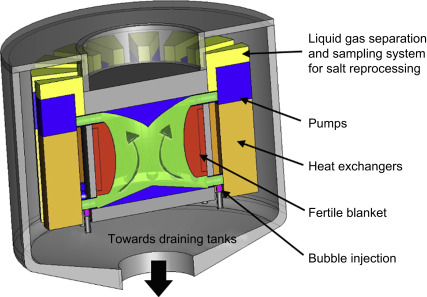
\includegraphics[width=.7\columnwidth]{msfr}
	\caption{Schematic diagram of the \gls{MSFR}. Retrieved from 
	\cite{allibert_7_2016}.}
	\label{fig:msfr}
\end{figure}

China and India have also started national programs supporting \gls{MSR}
development. China launched their \gls{TMSR} program in 2011 to develop and
construct both solid-fueled and liquid-fueled \gls{TMSR} designs
\cite{zou_research_2019}. Latest updates at the time of writing indicate that a
2-MW liquid-fueled prototype will complete construction by August
2021, with tests expected to start the following month. This milestone places
China ahead of other groups in the context of modern \gls{MSR} \gls{RD}
efforts. India also signaled their interest especially in thorium-based
reactors given their inherent and vast thorium reserves
\cite{jayaram_overview_1987}. They have developed conceptual designs of the
\gls{IMSBR}, expected to run on a fast/epithermal neutron spectrum to avoid
using graphite moderators given their tendency to deform under high neutron
fluence.

In the US, Southern Company received funding from \gls{DOE}'s
\gls{ARDP} \cite{doe_office_2021} to design, construct, and operate the
\gls{MCRE}, a prototype chloride salt-based \gls{MSR} relevant to TerraPower's
\gls{MCFR} \cite{terrapower_mcfr_2020}. This project builds on a prior
five-year cost-sharing project for the development of the \gls{MCFR} involving
TerraPower, Southern Company, Oak Ridge National Laboratory, Idaho National
Laboratory, the Electric Power Research Institute, and Vanderbilt University.
The \gls{MCFR} is a fast-spectrum \gls{MSR} similar to the \gls{MSFR}.
Canada-based Terrestrial Energy is also developing their \gls{IMSR}
\cite{leblanc_18_2017}, a small modular \gls{MSR} based on the \gls{MSRE}. The
replaceable \gls{IMSR} core-unit which holds the reactor core, pumps, heat
exchangers, and control rods, runs for approximately 7 years before it is shut
down and replaced after a cool-down period.

\gls{MSR} modeling software play an important role in supporting
\gls{MSR} development. They accelerate reactor design and optimization by
enabling engineers to iterate through numerous design changes. \gls{MSR}
modeling software are also essential tools in reactor safety analysis and
licensing efforts as engineers must demonstrate and verify their \gls{MSR}
designs remain safe under various accident scenarios. The next section
identifies challenges in \gls{MSR} multiphysics modeling with respect to
reactor accident analysis.

\section{Challenges in \gls{MSR} Multiphysics Modeling} \label{sec:challenges}

While modeling \glspl{MSR} is not necessarily more difficult than modeling
solid-fueled reactors, we must adapt our software tools to accurately model the
unique phenomena found in these circulating-fuel reactors. The differences in
the challenges of simulating \glspl{MSR} compared to solid-fueled reactors stem
mainly from the liquid fuel form of the fuel salt \cite{huff_identifying_2019,
diamond_phenomena_2018}.

Firstly, liquids generally exhibit greater thermal
expansion per unit change in temperature than solids. A decrease in density of
the fuel medium increases the likelihood of neutrons escaping the fuel region
and being absorbed by non-fissile material elsewhere in the reactor.
Consequently, combined with the temperature-dependent Doppler broadening of
resonance capture cross sections, \glspl{MSR} possess stronger negative fuel
temperature reactivity feedback than their solid-fueled counterparts
\cite{elsheikh_safety_2013}. These
phenomena ultimately result in strong interactions between the neutron fluxes
and core temperatures given that neutron fluxes affect core temperatures
through fission heat generation and core temperatures in turn affect neutron
fluxes through the mechanisms as described prior.

Secondly, with the fuel
salt also serving the role of providing cooling in the core, velocity flow
profiles in the fuel salts strongly impact the temperature distribution via
advection-dominated heat transfer \cite{diamond_phenomena_2018}. This contrasts
with the relatively static temperature distribution shapes in fuel pins and
other forms of solid fuel matrixes physically separated from the coolant; 
changes in coolant and the resultant changes in heat transfer rates in
solid-fueled reactors are often reduced to empirical correlations governing
convective heat transfer between the fuel cladding and the coolant. On the
other hand, the velocity flow profile has a more direct effect on the
temperature distribution and the temperature-dependent neutron cross sections
in \glspl{MSR}.

Lastly, \glspl{DNP} flow freely within the primary coolant loop as opposed to
being held in place as in solid-fueled reactors. Thus, the delayed neutron
source distribution varies significantly depending on the flow profile. In
addition,
the reactor loses some delayed neutrons from out-of-core \gls{DNP} decay. These
delayed neutrons are considered lost as they're emitted in subcritical regions
and are unlikely to contribute to further fission reactions. The reduced
delayed neutron fraction in the core strongly impacts the transient response of
the reactor in various accident scenarios. Thus, accurate \gls{MSR} transient
simulations require accurate modeling of \gls{DNP} drift.

As a result, multiphysics
software must employ \textit{tight coupling schemes} to couple the neutronics
and thermal-hydraulics governing equations to accurately capture the strong
multiphysics interactions in transient \gls{MSR} simulations. Tightly coupled
numerical models handle multiphysics interactions by either updating all state
variables simultaneously in one monolithic solve (\textit{full coupling}) or
iteratively updating all state variables (\textit{fixed point iterations})
until the solution converges in every timestep \cite{keyes_multiphysics_2013}.
Full coupling tends to be more computationally expensive because it combines
all physics equations into a single large system of equations to be solved
simultaneously, whereas fixed point iterations involve operator splitting to
separate the system of equations into smaller systems based on their associated
physics, solving smaller systems separately, and iteratively updating the state
variables until convergence. Fixed point iterative methods are often less
stable, less accurate, and have poorer
convergence rates since these methods make iterative corrections
without any regard to potentially destabilizing modes introduced by the
multiphysics coupling \cite{keyes_multiphysics_2013}. Notably, proven
techniques exist for improving the performance of fixed point iteration
coupling schemes for many relevant computational multiphysics research fields,
including reactor analysis \cite{ragusa_consistent_2009}. While fully coupled
schemes deal with solving a large system of equations, they can outperform
fixed point iterative methods in some multiphysics problems through superior
stability and convergence rates. 

In contrast to tight coupling schemes, \textit{loose coupling schemes}
solve each set of single-physics equations using state variable
data from the previous timestep without iterative corrections within every
timestep. Loosely coupled schemes are inappropriate for modeling \glspl{MSR}
given the strong coupling between the neutronics and thermal-hydraulics.
Aufiero et al. \cite{aufiero_development_2014} demonstrated a loose coupling
approach that failed to reproduce the expected increase in reactor power
in an \gls{MSR} in response to a 150 pcm reactivity insertion.

Consequently, most MSR multiphysics simulation tools employ, at
the very least, tight coupling schemes through fixed point iterations. The
next section explores various numerical coupling approaches in existing
multiphysics \gls{MSR} simulation tools.

\section{MSR Multiphysics Simulation Tools} \label{sec:msr-tools}

In recent years, several simulation tools have been developed for full-core
modeling of \glspl{MSR}. One approach involves coupling separate,
single-physics neutronics and thermal-hydraulics software. For example,
researchers at the Delft University of Technology coupled 3D neutron diffusion
software DALTON \cite{boer_validation_2010} and CFD software HEAT
\cite{de_zwaan_static_2007} to perform a safety analysis of the \gls{MSFR}
\cite{fiorina_modelling_2014}. In a later effort from the same institute,
Tiberga et al. \cite{tiberga_discontinuous_2019} coupled \gls{DG}-based
neutronics and thermal-hydraulics software, PHANTOM-$S_N$
and DGFlows, in their participation in the \gls{CNRS} Benchmark study
\cite{tiberga_results_2020}. Another multiphysics
package was developed at the \gls{PSI} coupling
thermal-hydraulics system software TRACE \cite{nrc_trace_2007} with the nodal
neutron diffusion software PARCS \cite{downar_parcs_2010} for the safety
analysis of the \gls{MSFR} \cite{pettersen_coupled_2016}. As such, one
advantage of coupling single-physics software to form an
integrated multiphysics tool is that it allows leverage of older,
well-validated single-physics software. These single-physics software are also
highly optimized for solving specific types of \glspl{PDE} relevant to their
respective physics.

With modern advancements in computing hardware and growing access to
high-performance computing, others have developed multiphysics tools by
coupling CFD software
OpenFOAM with Monte Carlo particle transport software Serpent 2, thus allowing
for high-fidelity neutronics calculations in transient reactor analyses.
Laureau et al. \cite{laureau_transient_2017} developed an innovative technique
called the \gls{TFM} method through the introduction of additional
time-dependence operators to conventional fission matrices typically used to
accelerate source convergence in Monte Carlo neutronics solves. The technique
uses Serpent 2 to pre-calculate three \glspl{TFM} of the reactor system and
interpolating the matrices during the actual transient calculations to
incorporate the effects of temperature-induced density change and Doppler
effect on the neutron cross sections and ultimately the neutron flux. Blanco
\cite{blanco_neutronic_2020} took a more computationally intensive approach of
compiling Serpent 2 as an internal \texttt{C}-based function within OpenFOAM's
\texttt{C++}-based framework. This approach reduced the amount of required data
transfers between Serpent 2 and OpenFOAM as both software have access to shared
memory during runtime. Their integrated tool employs the Quasi-Static
method for transient neutronics calculations and runs Serpent 2 Monte Carlo
calculations several times per timestep until convergence is reached.

The other approach towards creating \gls{MSR} simulation tools involves
developing inherently multiphysics software which can perform both
neutronics and thermal-hydraulics calculations. Among earlier efforts,
Nicolino et al. \cite{nicolino_coupled_2008} and Zhang et al.
\cite{zhang_development_2009} recognized the
need for more robust multiphysics coupling techniques and higher-fidelity
thermal hydraulics solutions to accurately capture complex flow profiles in
pool-type \glspl{MSR}. They each independently developed unnamed multiphysics
simulation tools and demonstrated their tools with non-moderated \gls{MSR}
designs. Later, Li et al. \cite{li_transient_2015} demonstrated the steady
state and transient analysis capabilities of COUPLE, a neutronics and
thermal-hydraulics software developed at the Karlsruhe Institute of Technology. 

Others opted to leverage general multiphysics software platforms such as
COMSOL \cite{comsol_ab_comsol_2018}, OpenFOAM \cite{openfoam_openfoam_2021},
and \gls{MOOSE} \cite{permann_moose_2020}. Researchers at Politecnico di
Milano developed a COMSOL-based \gls{MSR} simulation tool and modeled the
\gls{MSBR} as a single axisymmetric fuel channel with a uniform flow profile
\cite{cammi_multi-physics_2011}, followed by the \gls{MSRE} core also as a
single axisymmetric fuel channel with parabola-shaped laminar flow
\cite{cammi_dimensional_2012}. They expanded on their approach by modeling the
\gls{MSRE} upper plenum, downcomer and lower plenum, primary heat exchanger,
and secondary heat exchanger as 0D systems (lumped-parameter model), and
substituting the 2D fuel channel with a 3D fuel channel which more closely
resembled the actual fuel channels in the \gls{MSRE}
\cite{zanetti_geometric_2015}. Beyond graphite-moderated \glspl{MSR}, they've
also modeled the \gls{MSFR} in the same publication which featured Delft
University of Technology's DALTON + HEAT coupled multiphysics tool described
above. More recently, several European institutes (\gls{CNRS}, Politecnico di
Milano, and \gls{PSI}) have also developed coupled neutronics and
thermal-hydraulics tools in OpenFOAM. Their tools share some
similarities such as implementing the $SP_N$ simplified $P_N$ neutron transport
model and leveraging OpenFOAM's turbulent flow modeling capabilities.
Differences include the aforementioned external coupling capability with
Serpent 2 from \gls{CNRS} \cite{blanco_neutronic_2020}, fuel
compressibility modeling and helium bubble tracking capability from Politecnico
di Milano \cite{cervi_development_2019}, and fuel performance analysis
capability from \gls{PSI} \cite{fiorina_creation_2018}.

Finally, within the open-source, finite-element, multiphysics framework, MOOSE,
simulation tools capable of modeling
\glspl{MSR} include Moltres \cite{lindsay_moltres_2017}, the subject of
this work, and Rattlesnake \cite{wang_rattlesnake_2021}. Abou-Jaoude et al.
\cite{abou-jaoude_coupled_2020} coupled Rattlesnake with Pronghorn, another
MOOSE-based application for advanced reactor thermal-hydraulics modeling, to
demonstrate several steady-state \gls{MSR} simulation capabilities defined in
the \gls{CNRS} numerical benchmark. Lindsay et al.
\cite{lindsay_introduction_2018} first demonstrated Moltres' \gls{MSR} modeling
capabilities on 2D axisymmetric and 3D models of the \gls{MSRE} with fixed
velocity flow on a fully coupled neutronics and thermal-hydraulics solve. I
later demonstrated Moltres' more recent developments through modeling a 2D
axisymmetric model of the \gls{MSFR} for steady-state operation and transient
accident analysis \cite{park_advancement_2020}. The latter work introduces
looped \gls{DNP} flow, coupling the \gls{DNP} drift and temperature 
advection-diffusion to incompressible flow, and decay heat modeling
capabilities. The proposed work aims to continue Moltres development for
multiphysics \gls{MSR} analysis. The following chapter describes Moltres and
its existing capabilities for reactor analysis.
